

\tikzset{every picture/.style={line width=0.75pt}} %set default line width to 0.75pt        

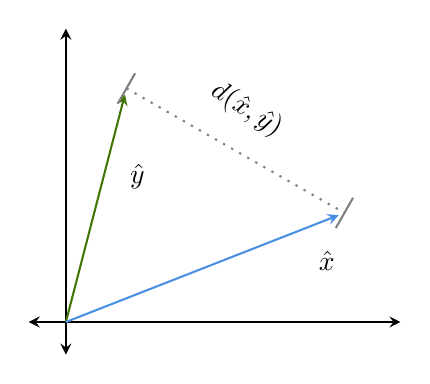
\begin{tikzpicture}[x=0.75pt,y=0.75pt,yscale=-1,xscale=1, scale=1.5]
%uncomment if require: \path (0,300); %set diagram left start at 0, and has height of 300

%Shape: Axis 2D [id:dp2895144271926746] 
\draw[stealth-stealth](48.6,95.03) -- (168,95.03);
\draw[stealth-stealth](60.54,0.83) -- (60.54,105.5);
%Straight Lines [id:da012847358875807346] 
\draw [color={rgb, 255:red, 65; green, 117; blue, 5 }  ,draw opacity=1, -stealth]   (60.54,95.03) -- (79.5,21.94) ;
%Straight Lines [id:da4678990026795582] 
\draw [color={rgb, 255:red, 74; green, 144; blue, 226 }  ,draw opacity=1, -stealth]   (60.54,95.03) -- (148.14,60.73) ;
%Straight Lines [id:da42874013324357696] 
\draw [color={rgb, 255:red, 128; green, 128; blue, 128 }  ,draw opacity=1 ] [dash pattern={on 0.84pt off 2.51pt}]  (80,20) -- (150,60) ;
\draw [shift={(150,60)}, rotate = 209.74] [color={rgb, 255:red, 128; green, 128; blue, 128 }  ,draw opacity=1 ][line width=0.75]    (0,5.59) -- (0,-5.59)   ;
\draw [shift={(80,20)}, rotate = 209.74] [color={rgb, 255:red, 128; green, 128; blue, 128 }  ,draw opacity=1 ][line width=0.75]    (0,5.59) -- (0,-5.59)   ;

% Text Node
\draw (140.82,71.3) node [anchor=north west][inner sep=0.75pt]    {$\hat{x}$};
% Text Node
\draw (80.16,43.4) node [anchor=north west][inner sep=0.75pt]    {$\hat{y}$};
% Text Node
\draw (110,15) node [anchor=north west][inner sep=0.75pt]  [rotate=-32.17]  {$\operatorname{d}(\hat{x} ,\hat{y})$};


\end{tikzpicture}
